\begin{singlespace}
    \chapter{\textbf{Soil nitrogen availability modifies leaf nitrogen economies in mature temperate deciduous forests: a direct test of photosynthetic least-cost theory}}
\end{singlespace}
    
\section{Introduction}
\noindent Photosynthesis represents the largest carbon flux between the atmosphere and land surface \shortcite{IPCC2021}, and plays a central role in biogeochemical cycling at multiple spatial and temporal scales \shortcite{Vitousek1991,LeBauer2008,Kaiser2015,Wieder2015_NPP}. Therefore, carbon and energy fluxes simulated by terrestrial biosphere models are sensitive to the formulation of photosynthetic processes \shortcite{Ziehn2011,Bonan2011,Booth2012,Smith2016,Smith2017} and must be represented using robust, empirically tested processes \shortcite{Prentice2015,Wieder2019}. Current formulations of photosynthesis vary across terrestrial biosphere models \shortcite{Smith2013,Rogers2017a}, which causes variation in modeled ecosystem processes \shortcite{Knorr2000,KnorrHeimann2001,Bonan2011,Friedlingstein2014} and casts uncertainty on the ability of these models to accurately predict terrestrial ecosystem responses and feedbacks to global change \shortcite{Zaehle2005,Schaefer2012,Davies-Barnard2020}.

Terrestrial biosphere models commonly represent C$_{3}$ photosynthesis th-rough variants of the \shortciteN{Farquhar1980} biochemical model \shortcite{Smith2013,Rogers2014,Rogers2017a}. This well-tested photosynthesis model estimates leaf-level carbon assimilation, or photosynthetic capacity, as a function of the maximum rate of Ribulose-1,5-bisphosphate carboxylase-oxygenase (Ru-bisco) carboxylation ($V_\mathrm{cmax}$) and the maximum rate of Ribulose-1,5-bisphosphate (RuBP) regeneration ($J_\mathrm{max}$) \shortcite{Farquhar1980}. Many terrestrial biosphere models predict these model inputs based on plant functional group specific linear relationships between leaf nutrient content and $V_\mathrm{cmax}$ \shortcite{Smith2013,Rogers2014,Rogers2017a} under the tenet that a large fraction of leaf nutrients, and nitrogen in particular, are partitioned toward building and maintaining enzymes that support photosynthetic capacity, such as Rubisco \shortcite{Brix1971,Gulmon1981,Evans1989_photoN,Kattge2009,Walker2014}. Terrestrial biosphere models predict leaf nutrient content from soil nutrient availability based on the assumption that increasing soil nutrients generally increases leaf nutrients \shortcite{Firn2019,Li2020,Liang2020} which, in the case of nitrogen, generally corresponds with an increase in photosynthetic processes \shortcite{Li2020,Liang2020}.

Recent work calls the generality of relationships between soil nutrient availability, leaf nutrient content, and photosynthetic capacity into question, suggesting instead that leaf nutrients and photosynthetic capacity are better predicted as an integrated product of aboveground climate, leaf traits, and soil nutrient availability, rather than soil nutrient availability alone \shortcite{Dong2017,Dong2020,Dong2022a,Firn2019,Smith2019,Peng2021}. It has been reasoned that this result is because plants allocate added nutrients to growth and storage rather than alterations in leaf chemistry \shortcite{Smith2019}, perhaps as a result of nutrient limitation of primary productivity \shortcite{LeBauer2008,Fay2015}. Additionally, recent work suggests that relationships between leaf nutrient content and photosynthesis vary across environments, and that the proportion of leaf nutrient content allocated to photosynthetic tissue varies over space and time with plant acclimation and adaptation responses to light availability, vapor pressure deficit, soil pH, soil nutrient availability, and environmental factors that influence leaf mass per area \shortcite{Pons1994,Niinemets1997,Evans2001,Hikosaka2009,Ghimire2017,Onoda2017,Luo2021}. The use of linear relationships between leaf nutrient content and $V_\mathrm{cmax}$ to predict photosynthetic capacity, as commonly used in terrestrial biosphere models \shortcite{Rogers2014}, is not capable of detecting such responses.

Photosynthetic least-cost theory provides an alternative framework for understanding relationships between soil nutrient availability, leaf nutrient content, and photosynthetic capacity \shortcite{Harrison2021}. Leveraging a two-input microeconomics approach \shortcite{Wright2003}, the theory posits that plants acclimate to a given environment by optimizing leaf photosynthesis rates at the lowest summed cost of using nutrients and water \shortcite{Prentice2014,Wang2017,Smith2019,Paillassa2020}. Across resource availability gradients, the theory predicts that optimal photosynthetic rates can be achieved by trading less efficient use of a resource that is less costly to acquire (or more abundant) for more efficient use of a resource more costly to acquire (or less abundant). For example, an increase in soil nutrient availability should reduce the cost of acquiring and using nutrients \shortcite{Bae2015,Eastman2021,Perkowski2021}, which could increase leaf nutrient investments in photosynthetic proteins to allow similar photosynthetic rates to be achieved with higher nutrient use (lower nutrient use efficiency) but lower water use (greater water use efficiency). The theory suggests similar tradeoffs in response to increasing soil pH \shortcite{Paillassa2020}, specifically, that increasing soil pH should reduce the cost of acquiring soil nutrients due to an increase in plant-available nutrient concentration \shortcite{Paillassa2020,Dong2022a}. The theory is also capable of reconciling dynamic leaf nutrient-photosynthesis relationships at global scales \shortcite{Luo2021}.

Patterns expected from photosynthetic least-cost theory have recently received empirical support both in global environmental gradient \shortcite{Smith2019,Paillassa2020,Luo2021,Querejeta2022,Westerband2023} and local manipulative invasion \shortcite{BialicMurphy2021} studies. However, nutrient addition experiments that directly examine nutrient-water use tradeoffs expected from the theory are rare (but see Guerrieri et al. 2011), and only global gradient studies testing the theory have considered soil pH in their analyses. As a result, there is a need to use nutrient addition and soil pH manipulation experiments to test mechanisms driving responses predicted by the theory.

In this study, I measured leaf responses to soil nitrogen availability in five deciduous tree species growing in the upper canopy of mature closed canopy temperate forests in the northeastern United States. Soil nitrogen availability and pH were manipulated through a nitrogen-by-pH field manipulation experiment with treatments applied since 2011, eight years prior to measurement. Two different soil nitrogen treatments were applied to increase nitrogen availability with opposing effects on soil pH. An additional nitrogen-free acidifying treatment was expected to decrease soil pH. I hypothesized that increased soil nitrogen availability would enable plants to increase nutrient uptake and create more photosynthetic enzymes per leaf, allowing similar photosynthetic rates achieved with lower leaf C$_\mathrm{i}$:C$_\mathrm{a}$ and increased leaf nitrogen content allocated to photosynthetic leaf tissue. I expected that this response would be driven by a reduction in the cost of acquiring nitrogen, which would cause trees to sacrifice efficient nitrogen use to enable more efficient use of other limiting resources (i.e., water). Finally, I hypothesized similar leaf responses to increasing soil pH.

\section{Methods}
\subsection{\textit{Study site description}}
\noindent I conducted this study in summer 2019 at three stands located within a 20-km radius of Ithaca, NY, USA (42.444 \textdegree{}N, 76.502 \textdegree{}W). All stands contain mature, closed-canopy forests dominated by deciduous tree species. Stands contained abundant sugar maple (\textit{Acer saccharum} Marshall), American beech (\textit{Fagus grandifolia} Ehrh.), and white ash (\textit{Fraxinus americana} L.), accounting for 43\%, 15\%, and 17\% of the total aboveground biomass across the three stands, respectively, with less frequent red maple (\textit{Acer rubrum} L.; 9\% of total aboveground biomass) and red oak occurrences (\textit{Quercus rubra} L.; 10\% of total aboveground biomass). Soils at each site were broadly classified as a channery silt loam Inceptisols using the USDA NRCS Web Soil Survey data product \shortcite{SoilSurveyStaff2022}. Between 2006 and 2020, study sites averaged 972 mm of precipitation per year and had an average temperature of 7.9 \textdegree{}C per a weather station located near the Cornell University campus (42.449 \textdegree{}N, 76.449 \textdegree{}W) part of the NOAA NCEI Global Historical Climatology Network \shortcite{Menne2012}.

\subsection{\textit{Experimental design}}
\noindent Four 40 m x 40 m plots were set up at each site in 2009, each with an additional 10 m buffer along plot perimeters (60 m x 60 m total). The plots were set up as a nitrogen-by-pH field manipulation experiment, with one each of four treatments at each site. Two nitrogen treatments were applied, both at 50 $\mathrm{kg\ N\ ha^{-1}\ yr^{-1}}$, as either sodium nitrate ($\mathrm{NaNO_3}$) to raise soil pH, or ammonium sulfate $\mathrm{((NH_4)_{2}SO_4)}$ to acidify; an elemental sulfur treatment was selected to acidify without nitrogen, applied at the same rate of S addition (57 $\mathrm{kg\ S\ ha^{-1}\ yr^{-1}}$); and control plots received no additions. All amendments were added in pelletized form using hand-held fertilizer spreaders to both the main plots and buffers. Amendments were divided into three equal doses distributed across the growing season from 2011-2017 and added as a single dose from 2018 onward. During 2019, plots were fertilized during the week of May 20.

\subsection{\textit{Leaf gas exchange and trait measurements}}
\noindent I sampled one leaf each from 6 to 10 individuals per plot between June 25 and July 12, 2019 for gas exchange measurements (Table \ref{table:tab.b1}). Leaves were collected from deciduous broadleaf trees represented across all sites and plots and were replicated in efforts to mimic the species abundance of each plot at each site. I attempted to collect leaves from the upper canopy to reduce differential shading effects on leaf physiology. Leaves were accessed by pulling down small branches using an arborist’s slingshot and weighted beanbag attached to a throw line. Branches were immediately recut under deionized water and remained submerged to reduce stomatal closure and avoid xylem embolism, as done in \shortciteN{Smith2018}, until gas exchange data were collected.

Randomly selected leaves with little to no visible external damage were attached to a Li-COR LI-6800 (Li-COR Bioscience, Lincoln, Nebraska, USA) portable photosynthesis machine to measure net photosynthesis ($A_\mathrm{net}$; $\mathrm{\mu mol\ m^{-2}}$ $\mathrm{{s}^{-1}}$), stomatal conductance ($g_\mathrm{sw}$; $\mathrm{mol\ m^{-2}\ s^{-1}}$), and intercellular CO$_2$ concentration ($C_\mathrm{i}$; $\mathrm{\mu mol\ mol^{-1}}$) at different reference CO$_2$ concentrations ($C_\mathrm{a}$; $\mathrm{\mu mol\ mol^{-1}}$) concentrations (i.e., an $A_\mathrm{net}/C_\mathrm{i}$ curve) under saturating light conditions (2,000 $\mathrm{\mu mol\ m^{-2}\ s^{-1}}$). Reference CO$_2$ concentrations followed the sequence: 400, 300, 200, 100, 50, 400, 400, 600, 800, 1000, 1200, 1500, and 2000 $\mathrm{\mu mol\ mol^{-1}\ CO_2}$. Leaf temperatures were not controlled in the cuvette and ranged from 21.8 \textdegree{}C to 31.7 \textdegree{}C (mean$\pm$SD: 27.2$\pm$2.2 \textdegree{}C). A linear and second order log-polynomial nonlinear regression suggested no effect of temperature on stomatal conductance measured at 400 $\mathrm{\mu mol\ mol^{-1}\ CO_2}$ or net photosynthesis measured at 400 $\mathrm{\mu mol\ mol^{-1}\ CO_2}$ (Table \ref{table:tab.b2}, \ref{table:tab.b3}; Fig. \ref{fig:figure.b1}). All $A_\mathrm{net}$/$C_\mathrm{i}$ curves were generated within one hour of branch severance.

Leaf morphological and chemical traits were collected on the same leaf used to generate each $A_\mathrm{net}/C_\mathrm{i}$ curve. Images of each leaf were taken using a flat-bed scanner to determine fresh leaf area using the ‘LeafArea’ R package \shortcite{Katabuchi2015}, which automates leaf area calculations using ImageJ software \shortcite{Schneider2012}. Each leaf was dried at 65\textdegree{}C for at least 48 hours, weighed, and ground using a Retsch MM200 ball mill grinder (Verder Scientific, Inc., Newtown, PA, USA) until homogenized. Leaf mass per unit leaf area ($M_\mathrm{area}$, g m$^{-2}$) was calculated as the ratio of dry leaf biomass to fresh leaf area. Using a subsample of ground and homogenized leaf biomass, leaf nitrogen content ($N_\mathrm{mass}$; gN g$^{-1}$) and leaf $\mathrm{\delta^{13}C}$ (‰, relative to Vienna Pee Dee Belemnite international reference standard) were measured at the Cornell Stable Isotope Lab with an elemental analyzer (NC 2500, CE Instruments, Wigan, UK) interfaced to an isotope ratio mass spectrometer (Delta V Isotope Ratio Mass Spectrometer, ThermoFisher Scientific, Waltham, MA, USA). Leaf nitrogen content per unit leaf area ($N_\mathrm{area}$; gN m$^{-2}$) was calculated by multiplying $N_\mathrm{mass}$ by $M_\mathrm{area}$.

I used leaf $\mathrm{\delta^{13}}$C values to estimate $\chi$ (unitless), which is an isotope-derived estimate of the leaf $C_\mathrm{i}$:$C_\mathrm{a}$ ratio. While intercellular and atmospheric CO$_2$ concentrations were directly measured during each $A_\mathrm{net}$/$C_\mathrm{i}$ curve, deriving $\chi$ from $\mathrm{\delta^{13}}$C provides a more integrative estimate of the leaf $C_\mathrm{i}$:$C_\mathrm{a}$ over an individual leaf’s lifespan. I derived $\chi$ following the approach of \shortciteN{Farquhar1989} described in \shortciteN{Cernusak2013}:

\begin{equation} \label{eq_2.1}
    \chi= \frac{\Delta^{13}C-a}{b-a}
\end{equation}

\noindent where $\mathrm{\Delta^{13}}$C represents the relative difference between leaf $\mathrm{\delta^{13}}$C (‰) and air $\mathrm{\delta^{13}}$C (‰), and is calculated from the following equation:

\begin{equation} \label{eq_2.2}
    \Delta^{13}C= \frac{\delta^{13}C_{air}-\delta^{13}C_{leaf}}{1+\delta^{13}C_{leaf}}
\end{equation}
    
\noindent where $\mathrm{\delta^{13}C_{air}}$ is assumed to be -8‰ \shortcite{Keeling1979,Farquhar1989}, \textit{a} represents the fractionation between $^{12}$C and $^{13}$C due to diffusion in air, assumed to be 4.4‰, and \textit{b} represents the fractionation caused by Rubisco carboxylation, assumed to be 27‰ \shortcite{Farquhar1989}.
    
\subsection{$A_{net}/C_i$ \textit{curve-fitting and parameter estimation}}
\noindent I fit $A_\mathrm{net}/C_\mathrm{i}$ curves of each individual using the ‘fitaci’ function in the ‘plantecophys’ R package \shortcite{Duursma2015}. This function estimates the maximum rate of Rubisco carboxylation ($V_\mathrm{cmax}$; $\mathrm{\mu mol\ m^{-2}\ s^{-1}}$) and maximum rate of electron transport for RuBP regeneration ($J_\mathrm{max}$; $\mathrm{\mu mol\ m^{-2}\ s^{-1}}$) based on the Farquhar, von Caemmerer, and Berry biochemical model of C$_{3}$ photosynthesis \shortcite{Farquhar1980}. For each curve fit, I included triose phosphate utilization (TPU) limitation to avoid underestimating $J_{\mathrm{max}}$ \shortcite{Gregory2021}. Curves were visually examined to confirm the likely presence of TPU limitation. 
    
I determined Michaelis-Menten coefficients for Rubisco affinity to CO$_2$ ($K_\mathrm{c}$; $\mathrm{\mu mol\ mol^{-1}}$) and $\mathrm{O_2}$ ($K_\mathrm{o}$; $\mathrm{\mu mol\ mol^{-1}}$), and the CO$_2$ compensation point ($\Gamma^*$; $\mathrm{\mu mol\ mol^{-1}}$) using leaf temperature and equations described in \shortciteN{Medlyn2002} and derived in \shortciteN{Bernacchi2001}. Specifically, $K_\mathrm{c}$ and $K_\mathrm{o}$ were calculated as:

\begin{equation} \label{eq_2.3}
    K_\mathrm{c}=404.9*exp^{\frac{79430(T_\mathrm{k}-298)}{298RT_\mathrm{k}}}
\end{equation}
    
\noindent and
    
\begin{equation} \label{eq_2.4}
    K_\mathrm{o}=278.4*exp^{\frac{36380(T_\mathrm{k}-298)}{298RT_\mathrm{k}}}
\end{equation}
    
\noindent while $\Gamma^*$ was calculated as:
    
\begin{equation} \label{eq_2.5}
    \Gamma^\mathrm{*}=42.75*exp^{\frac{37830(T_\mathrm{k}-298)}{298RT_\mathrm{k}}}
\end{equation}

\noindent In all three equations, $T_\mathrm{k}$ is the leaf temperature (in Kelvin) during each $A_\mathrm{net}/C_\mathrm{i}$ curve and R is the universal gas constant (8.314 J mol$^{-1}$ K$^{-1}$).

I standardized $V_\mathrm{cmax}$ and $J_\mathrm{max}$ estimates to 25 \textdegree{}C using a modified Arrhenius equation \shortcite{Kattge2007}:

\begin{equation} \label{eq_2.6}
    k_\mathrm{25}=\frac{k_\mathrm{obs}}{e^{\frac{H_a(T_{obs}-T_{ref})}{T_{ref}RT_{obs}}}*\frac{1+e^{\frac{T_{ref}\Delta S-H_d}{T_{ref}}}}{1+e^{\frac{T_{obs}\Delta S-H_d}{T_{obs}}}}}
\end{equation}

\noindent $k_\mathrm{25}$ represents the standardized $V_\mathrm{cmax}$ or $J_\mathrm{max}$ rate at 25\textdegree{}C, $k_\mathrm{obs}$ represents the $V_\mathrm{cmax}$ or $J_\mathrm{max}$ estimate at the average leaf temperature measured inside the cuvette during the $A_\mathrm{net}$/$C_\mathrm{i}$ curve. $H_\mathrm{a}$ is the activation energy of $V_{\mathrm{cmax}}$ (71,513 J mol$^{-1}$) \shortciteN{Kattge2007} or $J_\mathrm{max}$ (49,884 J mol$^{-1}$) \shortcite{Kattge2007}. $H_\mathrm{d}$ represents the deactivation energy of both $V_\mathrm{cmax}$ and $J_\mathrm{max}$ (200,000 J mol$^{-1}$) \shortcite{Medlyn2002}, and R represents the universal gas constant (8.314 J mol$^{-1}$ K$^{-1}$). $T_\mathrm{ref}$ represents the standardized temperature of 298.15 K (25\textdegree{}C) and $T_\mathrm{obs}$ represents the mean leaf temperature (in K) during each $A_\mathrm{net}$/$C_\mathrm{i}$ curve. $\Delta$S is an entropy term that \shortcite{Kattge2007} derived as a linear relationship with average growing season temperature ($T_\mathrm{g}$; \textdegree{}C), where: 

\begin{equation} \label{eq_2.7}
    \Delta S_{vcmax}=-1.07\ T_{g}+668.39
\end{equation}
    
\noindent and
   
\begin{equation} \label{eq_2.8}
    \Delta S_{jmax}=-0.75\ T_{g}+659.70
\end{equation}

\noindent I estimated $T_\mathrm{g}$ in Equations \ref{eq_2.7} and \ref{eq_2.8} based on mean daily (24-hour) air temperature of the 30 days leading up to the day of each sample collection using the same weather station reported in the site description. I used $V_\mathrm{cmax25}$ and $J_\mathrm{max25}$ estimates to calculate the ratio of $J_\mathrm{max25}$ to $V_\mathrm{cmax25}$ ($J_\mathrm{max25}$:$V_\mathrm{cmax25}$; unitless).

\subsection{\textit{Proportion of leaf nitrogen allocated to photosynthesis and structure}}
\noindent I used equations from \shortciteN{Niinemets1997} to estimate the proportion of leaf nitrogen content allocated to Rubisco and bioenergetics. The proportion of leaf nitrogen allocated to Rubisco ($\rho_\mathrm{rubisco}$; gN gN$^{-1}$) was calculated as a function of $V_\mathrm{cmax25}$ and $N_\mathrm{area}$: 

\begin{equation} \label{eqn_2.9}
    \rho_{rubisco}=\frac{V_{cmax25}N_r}{V_{cr}N_{area}}
\end{equation}

\noindent where $N_\mathrm{r}$ is the amount of nitrogen in Rubisco, set to 0.16 $\mathrm{gN\ (gN\ in\ Rubisco)^{-1}}$ and $V_\mathrm{cr}$ is the maximum rate of RuBP carboxylation per unit Rubisco protein, set to 20.5 $\mathrm{\mu mol\ CO_2\ (g\ Rubisco)^{-1}}$. The proportion of leaf nitrogen allocated to bioenergetics ($\mathrm{\rho_{bioe}}$; gN gN$^{-1}$) was similarly calculated as a function of $J_\mathrm{max25}$ and $N_\mathrm{area}$:

\begin{equation} \label{eqn_2.10}
    \rho_{bioe}=\frac{J_{max25}N_b}{J_{mc}N_{area}}
\end{equation}

\noindent where $N_\mathrm{b}$ is the amount of nitrogen in cytochrome f, set to 0.12407 gN ($\mu\mathrm{mol}$ cytochrome f)$^{-1}$ assuming a constant 1: 1: 1.2 cytochrome f: ferredoxin NADP reductase: coupling factor molar ratio \shortcite{EvansSeemann1989,Niinemets1997}, and $J_\mathrm{mc}$ is the capacity of electron transport per cytochrome f, set to 156 $\mathrm{\mu mol\ electron\ (\mu mol\ cytochrome\ f)^{-1} s^{-1}}$.

I estimated the proportion of leaf nitrogen content allocated to photosynthetic tissue ($\rho_\mathrm{photo}$; gN gN$^{-1}$) as the sum of $\rho_\mathrm{rubisco}$ and $\rho_\mathrm{bioe}$. This calculation is an underestimate of the proportion of leaf nitrogen allocated to photosynthetic tissue because it does not include nitrogen allocated to light harvesting proteins. This leaf nitrogen pool was not included because I did not perform chlorophyll extractions on focal leaves. However, the proportion of leaf nitrogen content allocated to light harvesting proteins tends to be small relative to $\rho_\mathrm{rubisco}$ and $\rho_\mathrm{bioe}$, and may scale with changes in $\rho_\mathrm{rubisco}$ and $\rho_\mathrm{bioe}$ \shortcite{Niinemets1997}.

Finally, the proportion of leaf nitrogen content allocated to structural tissue ($\rho_\mathrm{structure}$; gN gN$^{-1}$) was estimated as:
\begin{equation} \label{eqn_3.11}
    \rho_{structure}=\frac{N_{cw}}{N_{area}}
\end{equation}
\noindent where $N_\mathrm{cw}$ is the leaf nitrogen content allocated to cell walls (gN m$^{-2}$), calculated as a function of $M_\mathrm{area}$ using an empirical equation from \shortciteN{Onoda2017}:
\begin{equation} \label{eqn_3.12}
    N_{cw}=0.000355*{M_{area}}^{1.39}
\end{equation}


\subsection{\textit{Tradeoffs between nitrogen and water use}}
\noindent Photosynthetic nitrogen use efficiency (PNUE; $\mathrm{\mu mol\ CO_2\ mol^{-1}\ N\ s^{-1}}$) was calculated by dividing $A_\mathrm{net}$ by $N_\mathrm{area}$, first converting $N_\mathrm{area}$ to $\mathrm{mol\ N\ m^{-2}}$ using the molar mass of nitrogen (14 $\mathrm{g\ mol^{-1}}$). I used $\chi$ as an indicator of water use efficiency, which exploratory analyses suggest had similar responses to soil nitrogen availability and pH as intrinsic water use efficiency measured from gas exchange ($A_\mathrm{net}$/$g_\mathrm{sw}$). Tradeoffs between nitrogen and water use were determined by calculating the ratio of $N_\mathrm{area}$ to $\chi$ ($N_\mathrm{area}$:$\chi$; gN m$^{-2}$) and $V_\mathrm{cmax25}$ to $\chi$ ($V_\mathrm{cmax25}$:$\chi$; $\mathrm{\mu mol\ m^{-2}\ s^{-1}}$). This approach is similar to tradeoff calculations in which nitrogen-water use tradeoffs are measured as the ratio of $N_\mathrm{area}$ or $V_\mathrm{cmax25}$ to $g_\mathrm{sw}$ \shortcite{Paillassa2020,BialicMurphy2021}. In this chapter, I quantify these relationships using $\chi$ in lieu of $g_\mathrm{sw}$ because $g_\mathrm{sw}$ rapidly changes with environmental conditions and therefore may have been altered by recent tree branch severance and/or placement in the cuvette.

\subsection{\textit{Soil nitrogen availability and pH}}
\noindent To characterize soil nitrogen availability at the time of our leaf gas exchange measurements, I used mixed bed resin bags to quantify mobile ammonium-N and nitrate-N concentrations in each plot. Lycra mesh bags were filled with 5 g of Dowex\textregistered\ Marathon MR-3 hydrogen and hydroxide form resin (MilliporeSigma, Burlington, MA USA) and sealed with a zip tie. Each bag was activated by soaking in 0.5 M HCl for 20 minutes, then in 2 M NaCl until pH of the saline solution stabilized, as described in \shortciteN{Allison2008a}. Five resin bags were inserted about 10 cm below the soil surface at each plot on June 25, 2019: one near each of the four plot corners and one near the plot center. All resin bags were collected 24 days later on July 19, 2019 and were frozen until extracted.
    
Prior to anion and cation extraction, each resin bag was rinsed with ultrapure water (MilliQ IQ 7000; Millipore Sigma, Burlington, MA) to remove any surface soil residues. Anions and cations were extracted from surface-cleaned resin bags by individually soaking and shaking each bag in 100 mL of a 0.1 M HCl/2.0 M NaCl matrix for one hour. Using a microplate reader (Biotek Synergy H1; Biotek Instruments, Winooski, VT USA), I quantified nitrate-N concentrations spectrophotometrically at 540 nm with the end product of a single reagent vanadium (III) chloride reaction \shortcite{Doane2003}, and ammonium-N concentrations quantified at 650 nm with the end product of a modified phenol-hypochlorite reaction \shortcite{Weatherburn1967,Rhine1998}. Both the single reagent vanadium (III) chloride and modified phenol-hypochlorite methodologies are well established for determining nitrate-N and ammonium-N concentrations in resin bag extracts \shortcite{Arnone1997,Allison2008a}. I used a series of negative and positive controls throughout each well plate to verify the accuracy and precision of our measurements, assaying each resin bag extract and control in triplicate. Soil nitrogen availability was estimated as the sum of the nitrate-N and ammonium-N concentration in each resin bag, normalized per g of resin and duration in the field ($\mathrm{\mu g\ N\ g^{-1}\ resin\ d^{-1}}$), then subsequently averaged across all resin bags in a plot for a plot-level mean.
    
Soil pH was measured on 0-10 cm mineral soil samples collected prior to fertilization in 2019. Near each of the four plot corners, three 5.5 cm diameter soil cores were collected after first removing the forest floor where present. Each set of three cores was placed in a plastic bag, and later composited by hand mixing and sieved to 4mm. Soil pH was determined for a 1:2 soil:water slurry (10 g field-moist soil to 20 mL DI water) of each sample using an Accumet AB15 pH meter with flushable junction probe (Fisher Scientific; Hampton, NH, USA), and was estimated at the plot level as the mean soil pH within each plot.

\subsection{\textit{Statistical analyses}}
\noindent I built two separate series of linear mixed-effects models to explore effects of soil nitrogen availability, soil pH, species, and leaf nitrogen content on leaf physiological traits. In the first series of linear mixed-effects models, I explored the effect of soil nitrogen availability, soil pH, and species on leaf nitrogen content, leaf photosynthesis, stomatal conductance, and nitrogen-water use tradeoffs. Models included plot-level soil nitrogen availability and plot-level soil pH as continuous fixed effects, species as a categorical fixed effect, and site as a categorical random intercept term. Interaction terms between fixed effects were not included due to the small number of experimental plots. I built a series of separate models with this independent variable structure to quantify individual effects of soil nitrogen availability, soil pH, and species on $N_\mathrm{area}$, $M_\mathrm{area}$, $N_\mathrm{mass}$, $A_\mathrm{net}$, $V_\mathrm{cmax25}$, $J_\mathrm{max25}$, $J_\mathrm{max25}$:$V_\mathrm{cmax25}$, $\rho_\mathrm{rubisco}$, $\rho_\mathrm{bioenergetics}$, $\rho_\mathrm{photo}$, $\rho_\mathrm{structure}$, $\chi$, PNUE, $N_\mathrm{area}$:$\chi$, and $V_\mathrm{cmax25}$:$\chi$.

A second series of linear mixed-effects models were built to investigate relationships between leaf nitrogen content and photosynthetic parameters. Statistical models included $N_\mathrm{area}$ as a single continuous fixed effect with species and site designated as individual random intercept terms. I used this independent variable structure to quantify individual effects of leaf nitrogen content on $A_\mathrm{net}$, $V_\mathrm{cmax25}$, $J_\mathrm{max25}$, $J_\mathrm{max25}$:$V_\mathrm{cmax25}$, and $\chi$.

For all linear mixed-effects models, I used Shapiro-Wilk tests of normality to determine whether linear mixed-effects models satisfied residual normality assumptions. If residual normality assumptions were not met, then models were fit using dependent variables that were natural log transformed. If residual normality assumptions were still not met (Shapiro-Wilk: \textit{p}<0.05), then models were fit using dependent variables that were square root transformed. All residual normality assumptions for both sets of models that did not originally satisfy residual normality assumptions were met with either a natural log or square root data transformation (Shapiro-Wilk: \textit{p}>0.05 in all cases).

In the first series of models, models for $N_\mathrm{area}$, $M_\mathrm{area}$, $N_\mathrm{mass}$, $V_\mathrm{cmax25}$, $J_\mathrm{max25}$, $\chi$, $N_{\mathrm{area}}$:$\chi$, and $V_\mathrm{cmax25}$:$\chi$, $\rho_\mathrm{rubisco}$, $\rho_\mathrm{bioenergetics}$, $\rho_\mathrm{photo}$, $\rho_\mathrm{structure}$ satisfied residual normality assumptions without data transformations (Shapiro-Wilk: \textit{p}>0.05 in all cases). The model for $J_\mathrm{max25}$:$V_\mathrm{cmax25}$ satisfied residual normality assumptions with a natural log data transformation, while models for $A_\mathrm{net}$ and PNUE each satisfied residual normality assumptions with square root data transformations. In the second series of models, models for $V_\mathrm{cmax25}$, $J_\mathrm{max25}$, $\chi$, and $V_\mathrm{cmax25}$:$\chi$ satisfied residual normality assumptions without data transformations (Shapiro-Wilk: \textit{p}>0.05 in all cases). The model for $J_\mathrm{max25}$:$V_\mathrm{cmax25}$ required a natural log data transformation and the model for $A_\mathrm{net}$ required a square root data transformation (Shapiro-Wilk: \textit{p}>0.05 in both cases).
    
In all models, I used the ‘lmer’ function in the ‘lme4’ R package \shortcite{Bates2015} to fit each model and the ‘Anova’ function in the ‘car’ R package \shortcite{Fox2019} to calculate Type II Wald’s $\chi^2$ and determine the significance level ($\alpha$=0.05) of each fixed effect coefficient. Finally, I used the ‘emmeans’ R package (Lenth, 2019) to conduct post-hoc comparisons using Tukey’s tests, where degrees of freedom were approximated using the Kenward-Roger approach \shortcite{Kenward1997}. All analyses and plots were conducted in R version 4.1.1 \shortcite{RCoreTeam2021}. All figure regression lines and associated 95\% confidence interval error bars were plotted using predictions generated across the soil nitrogen availability gradient using the ‘emmeans’ R package \shortcite{Lenth2019}.
    
\section{Results}
\subsection{\textit{Leaf nitrogen content}}  
\noindent Increasing soil nitrogen availability generally increased $N_\mathrm{area}$ (Table \ref{tab:table3.1}; Fig. \ref{fig:figure3.1}a). This pattern was driven by an increase in $N_\mathrm{mass}$ (Table \ref{tab:table3.1}; Fig. \ref{fig:figure3.1}c) and a marginal increase in $M_\mathrm{area}$ (Table \ref{tab:table3.1}; Fig. \ref{fig:figure3.1}e) with increasing soil nitrogen availability. There was no effect of soil pH on $N_\mathrm{area}$, $N_\mathrm{mass}$, or $M_\mathrm{area}$ (Table \ref{tab:table3.1}); however, I also observed strong differences in $N_\mathrm{area}$ (Fig. \ref{fig:figure3.1}b), $N_\mathrm{mass}$ (Fig. \ref{fig:figure3.1}d), and $M_\mathrm{area}$ (Fig. \ref{fig:figure3.1}e) between species (Table \ref{tab:table3.1}).
    \clearpage

    \newpage
    \begin{landscape}
        \begin{table}[]
        \centering
        \caption[Effects of soil nitrogen availability, soil pH, and species on leaf nitrogen content per unit leaf area, leaf nitrogen content per unit leaf mass, and leaf mass per unit leaf area]{Effects of soil nitrogen availability, soil pH, and species on leaf nitrogen content per unit leaf area ($N_\mathrm{area}$; gN m$^{-2}$), leaf nitrogen content per unit leaf mass ($N_\mathrm{mass}$; gN g$^{-1}$), and leaf mass per unit leaf area ($M_\mathrm{area}$; g m$^{-2}$)$^*$}
        \resizebox{\columnwidth}{!}{
        \begin{tabular}{p{2.5cm}p{0.5cm}p{2cm}p{1.5cm}p{1.5cm}p{2cm}p{1.5cm}p{1.5cm}p{2cm}p{1.5cm}p{1.5cm}}
                 && 
                 \multicolumn{3}{l}{$N_\mathrm{area}$} 
                 & \multicolumn{3}{l}{$N_\mathrm{mass}$} 
                 & \multicolumn{3}{l}{$M_\mathrm{area}$} 
                 \\
                 \hline 
                 & 
                 \multicolumn{1}{r}{df} 
                 & \multicolumn{1}{r}{Coefficient} & \multicolumn{1}{r}{$\chi^{2}$} & \multicolumn{1}{r}{\textit{p}} 
                 & \multicolumn{1}{r}{Coefficient} & \multicolumn{1}{r}{$\chi^{2}$} & \multicolumn{1}{r}{\textit{p}} 
                 & \multicolumn{1}{r}{Coefficient} & \multicolumn{1}{r}{$\chi^{2}$} & \multicolumn{1}{r}{\textit{p}} 
                 \\ 
                 \hline

                 Intercept & \multicolumn{1}{r}{-} 
                 &  \multicolumn{1}{r}{9.03E$-$01} & \multicolumn{1}{r}{-} & \multicolumn{1}{r}{-}
                 &  \multicolumn{1}{r}{1.68E+00} & \multicolumn{1}{r}{-} & \multicolumn{1}{r}{-}
                 &  \multicolumn{1}{r}{4.60E+01} & \multicolumn{1}{r}{-} & \multicolumn{1}{r}{-} 
                 \\

                 Soil N & \multicolumn{1}{r}{1}
                 & \multicolumn{1}{r}{1.68E$-$02} & \multicolumn{1}{r}{11.990} & \multicolumn{1}{r}{\textbf{0.001}}
                 & \multicolumn{1}{r}{1.25E$-$02}  & \multicolumn{1}{r}{6.902} & \multicolumn{1}{r}{\textbf{0.009}}
                 & \multicolumn{1}{r}{4.87E$-$01}  & \multicolumn{1}{r}{4.143} & \multicolumn{1}{r}{\textbf{0.042}} 
                 \\


                 Soil pH & \multicolumn{1}{r}{1}
                 & \multicolumn{1}{r}{9.28E$-$02} & \multicolumn{1}{r}{0.836} & \multicolumn{1}{r}{0.361}
                 & \multicolumn{1}{r}{8.08E$-$02} & \multicolumn{1}{r}{0.663} & \multicolumn{1}{r}{0.415}
                 & \multicolumn{1}{r}{4.05E+00} & \multicolumn{1}{r}{0.653} & \multicolumn{1}{r}{0.419} 
                 \\

                 Species & \multicolumn{1}{r}{4}
                 & \multicolumn{1}{r}{-} & \multicolumn{1}{r}{72.128} &  \multicolumn{1}{r}{\textbf{\textless{}0.001}}
                 & \multicolumn{1}{r}{-} & \multicolumn{1}{r}{35.074} &  \multicolumn{1}{r}{\textbf{\textless{}0.001}}
                 & \multicolumn{1}{r}{-} & \multicolumn{1}{r}{29.869} &  \multicolumn{1}{r}{\textbf{\textless{}0.001}}
                 \\
                 \hline

                 &&&&&&&&&& 
                 \\
    \end{tabular}}
    \label{tab:table3.1}
\end{table}
\begin{singlespace}
    \noindent $^*$Significance determined using Type II Wald $\chi^{2}$ tests ($\alpha$=0.05). \textit{P}-values<0.05 are in bold.       
\end{singlespace}
\end{landscape}
\clearpage

\newpage
\begin{figure}
    \includegraphics[scale = 0.055]{ch3_NxpH/figs/NxS_fig1_leafn.png}
    \centering
    \caption[Effects of soil nitrogen availability and species on leaf nitrogen content per unit leaf area, leaf nitrogen content per unit leaf biomass, and leaf mass per leaf area]{Effects of soil N availability and species on leaf nitrogen content per unit leaf area (a-b), leaf nitrogen content per unit leaf biomass (c-d), and leaf mass per leaf area (e-f). Soil nitrogen availability is represented on the x-axis in the left column of panels, while species is represented on the x-axis in the right column of panels. Tree species are represented as colored points and treatment plots are represented as shaped points, jittered for visibility. Species are abbreviated in the right column of panels through their assigned NRCS PLANTS Database symbol \shortcite{USDANRCS2022}, grouped along the x-axis per common mycorrhizal association, where the first three species commonly associate with arbuscular mycorrhizae (ACRU, ASCA, FAGR) and the second two species with ectomycorrhizae (FAGR, QURU). Trendlines are only included when the regression slope is statistically different from zero (\textit{p}<0.05).}
    \label{fig:figure3.1}
\end{figure}
\clearpage

\newpage
\subsection{\textit{Net photosynthesis and leaf biochemistry}}
\noindent Increasing soil nitrogen availability generally had no effect on $A_\mathrm{net}$, $V_\mathrm{cmax25}$, $J_\mathrm{max25}$, or $J_\mathrm{max25}$:$V_\mathrm{cmax25}$ (Table \ref{tab:table3.2}, Figs. \ref{fig:figure3.2}a, \ref{fig:figure3.2}d, \ref{fig:figure3.2}g). I also observed strong species effects on all measured leaf photosynthetic traits (Table \ref{tab:table3.2}; Figs. \ref{fig:figure3.2}b, \ref{fig:figure3.2}e, \ref{fig:figure3.2}h). Increasing soil pH had a marginal negative effect on $A_\mathrm{net}$, but had no effect on $V_\mathrm{cmax25}$, $J_\mathrm{max25}$, or $J_\mathrm{max25}$:$V_\mathrm{cmax25}$ (Table \ref{tab:table3.2}). There was a weak positive effect of increasing $N_\mathrm{area}$ on $A_\mathrm{net}$ (Fig. \ref{fig:figure3.2}c), but quite strong positive effects of increasing $N_\mathrm{area}$ on $V_\mathrm{cmax25}$ and $J_\mathrm{max25}$ (Table \ref{tab:table3.2}; Fig. \ref{fig:figure3.2}f and \ref{fig:figure3.2}i).
\clearpage
    
\newpage
\begin{landscape}
    \begin{table}
    \centering
    \caption[Effects of soil nitrogen availability, soil pH, species, and $N_\mathrm{area}$ on net photosynthesis, the maximum rate of Rubisco carboxylation, the maximum rate of RuBP regeneration, and the ratio of the maximum rate of RuBP regeneration to the maximum rate of Rubisco carboxylation]{Effects of soil nitrogen availability, soil pH, species, and $N_\mathrm{area}$ on net photosynthesis ($A_\mathrm{net}$; $\mathrm{\mu mol\ m^{-2}\ s^{-1}}$), the maximum rate of Rubisco carboxylation ($V_\mathrm{cmax25}$; $\mathrm{\mu mol\ m^{-2}\ s^{-1}}$), the maximum rate of RuBP regeneration ($J_\mathrm{max25}$; $\mathrm{\mu mol\ m^{-2}\ s^{-1}}$), and the ratio of the maximum rate of RuBP regeneration to the maximum rate of Rubisco carboxylation ($J_\mathrm{max25}$:$V_\mathrm{cmax25}$; unitless)$^*$}
    \resizebox{\columnwidth}{!}{
    \begin{tabular}{p{2.5cm}p{0.5cm}p{2cm}p{1.5cm}p{1.5cm}p{2cm}p{1.5cm}p{1.5cm}p{2cm}p{1.5cm}p{1.5cm}}
            && 
            \multicolumn{3}{l}{$A_\mathrm{net}$} 
            & \multicolumn{3}{l}{$V_\mathrm{cmax25}$} 
            & \multicolumn{3}{l}{$J_\mathrm{max25}$} 
            \\
            \hline 
            & 
            \multicolumn{1}{r}{df} 
            & \multicolumn{1}{r}{Coefficient} & \multicolumn{1}{r}{$\chi^{2}$} & \multicolumn{1}{r}{\textit{p}} 
            & \multicolumn{1}{r}{Coefficient} & \multicolumn{1}{r}{$\chi^{2}$} & \multicolumn{1}{r}{\textit{p}} 
            & \multicolumn{1}{r}{Coefficient} & \multicolumn{1}{r}{$\chi^{2}$} & \multicolumn{1}{r}{\textit{p}} 
            \\ 
            \hline

            (Intercept) & \multicolumn{1}{r}{-} 
            &  \multicolumn{1}{r}{3.29E+00$^\mathrm{b}$} & \multicolumn{1}{r}{-} & \multicolumn{1}{r}{-}
            &  \multicolumn{1}{r}{6.38E+01}                    & \multicolumn{1}{r}{-} & \multicolumn{1}{r}{-}
            &  \multicolumn{1}{r}{1.12E+02}                    & \multicolumn{1}{r}{-} & \multicolumn{1}{r}{-} 
            \\

            Soil N & \multicolumn{1}{r}{1}
            & \multicolumn{1}{r}{-1.23E$-$03$^\mathrm{b}$} & \multicolumn{1}{r}{1.798} & \multicolumn{1}{r}{0.180}
            & \multicolumn{1}{r}{-3.84E$-$01}                    & \multicolumn{1}{r}{1.745} & \multicolumn{1}{r}{0.187}
            & \multicolumn{1}{r}{-6.70E$-$01}                    & \multicolumn{1}{r}{2.172} & \multicolumn{1}{r}{0.141} 
            \\

            Soil pH & \multicolumn{1}{r}{1}
            & \multicolumn{1}{r}{-3.09E$-$01$^\mathrm{b}$} & \multicolumn{1}{r}{3.312} & \multicolumn{1}{r}{\textit{0.069}}
            & \multicolumn{1}{r}{-4.91E+00}                    & \multicolumn{1}{r}{0.655} & \multicolumn{1}{r}{0.418}
            & \multicolumn{1}{r}{-8.18E+00}                    & \multicolumn{1}{r}{0.742} & \multicolumn{1}{r}{0.389} 
            \\

            Species & \multicolumn{1}{r}{4}
            & \multicolumn{1}{r}{-} & \multicolumn{1}{r}{11.838} & \multicolumn{1}{r}{\textbf{0.019}}
            & \multicolumn{1}{r}{-} & \multicolumn{1}{r}{31.748} & \multicolumn{1}{r}{\textbf{\textless{}0.001}}
            & \multicolumn{1}{r}{-} & \multicolumn{1}{r}{27.291} & \multicolumn{1}{r}{\textbf{\textless{}0.001}}
            \\
            \hline

            ($N_\mathrm{area}$ int.) & \multicolumn{1}{r}{-}
            & \multicolumn{1}{r}{6.59E$-$01$^\mathrm{b}$} & \multicolumn{1}{r}{-} & \multicolumn{1}{r}{-}
            & \multicolumn{1}{r}{1.45E$-$01}                    & \multicolumn{1}{r}{-} & \multicolumn{1}{r}{-}
            & \multicolumn{1}{r}{2.86E+01}                    & \multicolumn{1}{r}{-} & \multicolumn{1}{r}{-}
            \\

            $N_\mathrm{area}$ & \multicolumn{1}{r}{4}
            & \multicolumn{1}{r}{3.13E$-$01$^\mathrm{b}$} & \multicolumn{1}{r}{4.790} & \multicolumn{1}{r}{\textbf{0.029}}
            & \multicolumn{1}{r}{2.43E+01}                    & \multicolumn{1}{r}{22.616} & \multicolumn{1}{r}{\textbf{\textless{}0.001}}
            & \multicolumn{1}{r}{4.04E+01}                    & \multicolumn{1}{r}{28.259} & \multicolumn{1}{r}{\textbf{\textless{}0.001}}
            \\
            \hline
            &&&&&&&&&&
            \\

            && \multicolumn{3}{l}{$J_\mathrm{max25}$:$V_\mathrm{cmax25}$} &&&&& \\
            \hline
            & \multicolumn{1}{r}{df}
            & \multicolumn{1}{r}{Coefficient} & \multicolumn{1}{r}{$\chi^{2}$} & \multicolumn{1}{r}{\textit{p}} 
            \\
            \hline

            (Intercept) & \multicolumn{1}{r}{-}
            & \multicolumn{1}{r}{6.59E$-$01$^\mathrm{a}$} & \multicolumn{1}{r}{-} & \multicolumn{1}{r}{-}
            &&&&&&
            \\

            Soil N & \multicolumn{1}{r}{1}
            & \multicolumn{1}{r}{7.04E$-$04$^\mathrm{a}$}  & \multicolumn{1}{r}{0.088} & \multicolumn{1}{r}{0.767}
            &&&&&& 
            \\

            Soil pH & \multicolumn{1}{r}{1}
            & \multicolumn{1}{r}{-7.84E$-$03$^\mathrm{a}$} & \multicolumn{1}{r}{0.025} & \multicolumn{1}{r}{0.874}
            &&&&&& 
            \\

            Species & \multicolumn{1}{r}{4}
            & \multicolumn{1}{r}{-} & \multicolumn{1}{r}{12.745} & \multicolumn{1}{r}{\textbf{0.013}} \\
            \hline

            ($N_\mathrm{area}$ int.) & \multicolumn{1}{r}{-}
            & \multicolumn{1}{r}{6.69E$-$01$^\mathrm{a}$} & \multicolumn{1}{r}{-} & \multicolumn{1}{r}{-}
            &&&&&& 
            \\

            $N_\mathrm{area}$ & \multicolumn{1}{r}{4}
            & \multicolumn{1}{r}{-4.69E$-$02$^\mathrm{a}$} & \multicolumn{1}{r}{1.142} & \multicolumn{1}{r}{0.285}
            &&&&& \\
            \hline
        \end{tabular}}
        \label{tab:table3.2}
    \end{table}
\begin{singlespace}
    \noindent \textsuperscript{$*$}Significance determined using Type II Wald $\chi^{2}$ tests ($\alpha$=0.05). \textit{P}-values less than 0.05 are in bold, while \textit{p}-values between 0.05 and 0.1 are italicized. Superscript letters indicate model coefficients fit to natural-log ($^\mathrm{a}$) or square-root ($^\mathrm{b}$) transformed data. Relationships between $N_\mathrm{area}$ and each response variable were fit using the second series of bivariate mixed-effects models, so model coefficients and results are independent of model coefficients and results reported for relationships between soil nitrogen, soil pH, and species for each response variable.
\end{singlespace}
\end{landscape}
\clearpage

\newpage
\begin{figure}
    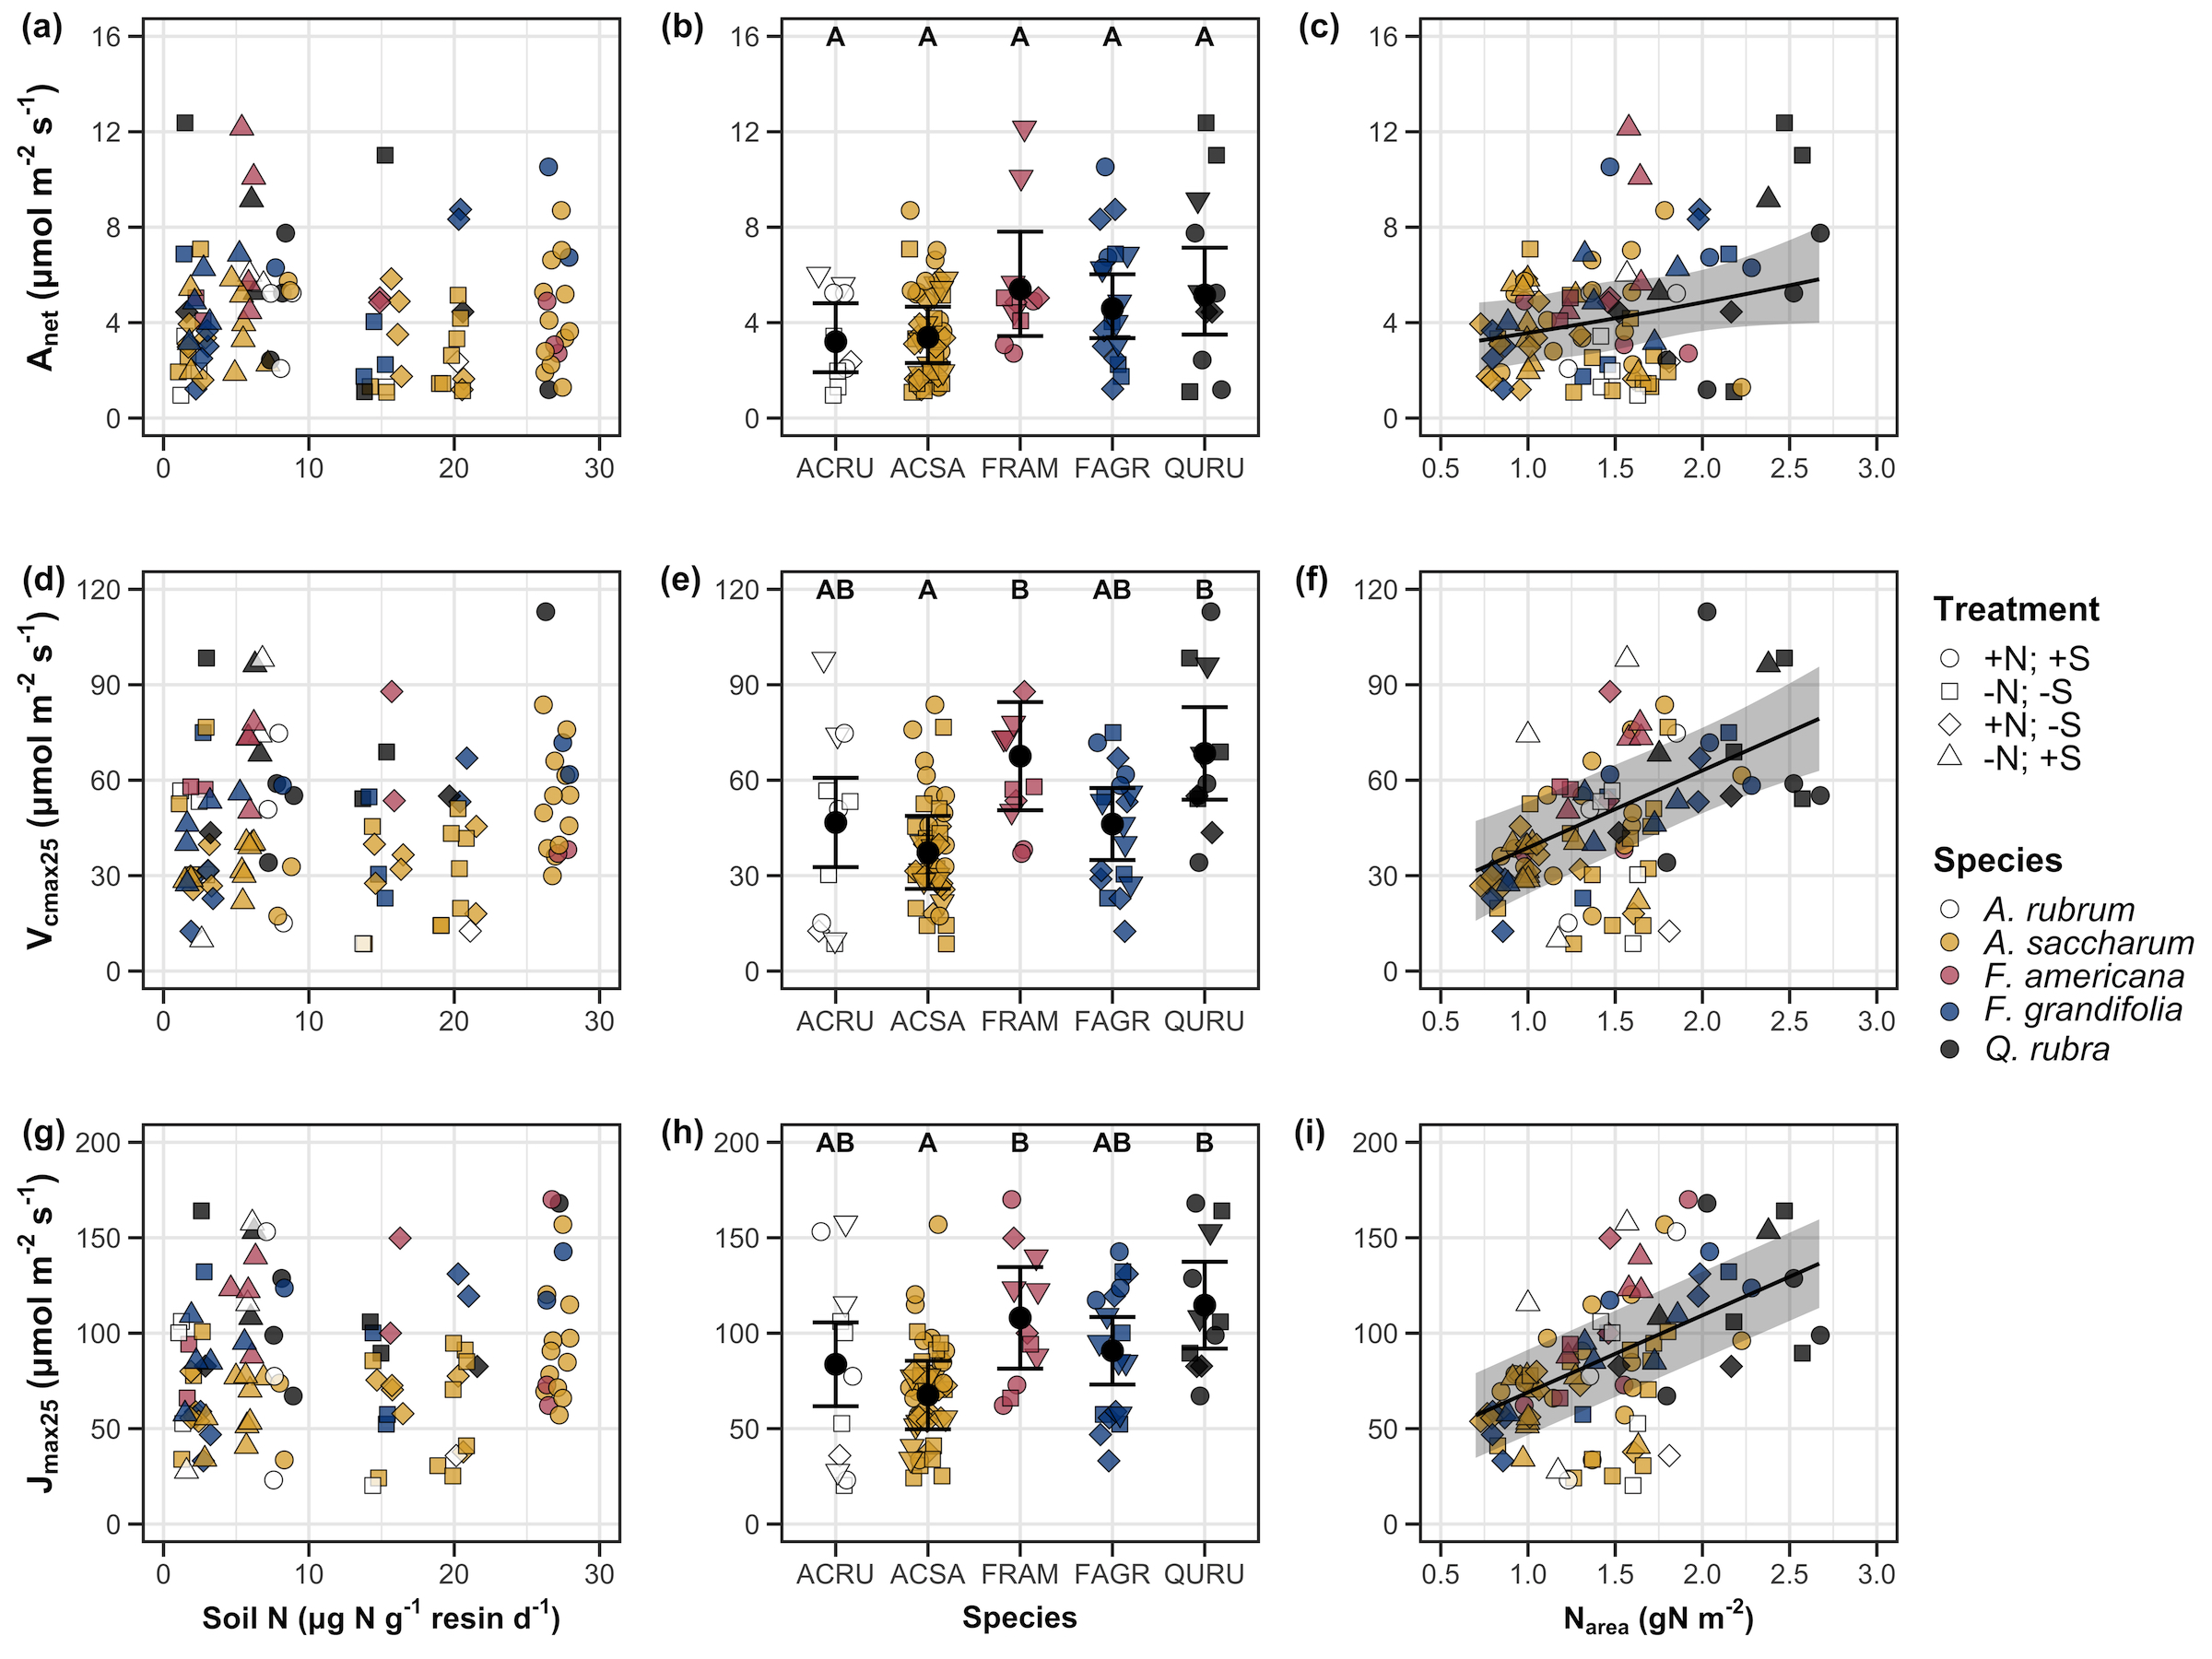
\includegraphics[width=\textwidth]{ch3_NxpH/figs/NxS_fig2_leafbiochem.png}
    \centering
    \caption[Effects of soil nitrogen availability, species, and leaf nitrogen content on net photosynthesis, maximum Rubisco carboxylation rate, and maximum RuBP regeneration rate]{Effects of soil nitrogen availability (left column of panels), species (middle column of panels), and leaf nitrogen content per unit leaf area (right column of panels) on net photosynthesis (a-c), maximum Rubisco carboxylation rate (d-f), and maximum RuBP regeneration rate (g-i). Soil nitrogen availability is represented on the x-axis in the left column of panels, species is represented on the x-axis in the middle column of panels, and leaf nitrogen content per unit leaf area is represented continuously on the x-axis in the right column of panels. Species abbreviations and position along the x-axis in the middle column of panels, colored points, shapes, and trendlines are as explained in Figure \ref{fig:figure3.1}.}
    \label{fig:figure3.2}
\end{figure}
\clearpage

\newpage
\subsection{\textit{Leaf nitrogen allocation}}
\noindent Neither soil nitrogen availability nor soil pH affected the proportion of leaf nitrogen allocated to Rubisco or bioenergetics (Table \ref{tab:table3.3}; Fig. \ref{fig:figure3.3}a, Fig. \ref{fig:figure3.3}c). There was also no effect of soil nitrogen availability or soil pH on the proportion of leaf nitrogen allocated to photosynthesis (Table \ref{tab:table3.3}; Fig. \ref{fig:figure3.3}f). I found no effect of soil nitrogen availability or soil pH on the proportion of leaf nitrogen allocated to structure (Table \ref{tab:table3.3}; Fig \ref{fig:figure3.3}g). Species varied in the proportion of leaf nitrogen allocated to Rubisco, photosynthesis, and structure (Fig \ref{fig:figure3.3}b, Fig. \ref{fig:figure3.3}f, Fig \ref{fig:figure3.3}h), with no detectable species effect on the proportion of leaf nitrogen allocated to bioenergetics (Table \ref{tab:table3.3}, Fig. \ref{fig:figure3.3}d).
\clearpage

\newpage
\begin{landscape}
    \begin{table}
    \centering
    \caption[Effects of soil nitrogen availability, soil pH, and species on the proportion of leaf nitrogen content allocated to photosynthesis, Rubisco, bioenergetics, and structure]{Effects of soil nitrogen availability, soil pH, and species on the proportion of leaf nitrogen content allocated to photosynthesis ($\rho_\mathrm{photo}$; gN gN$^{-1}$), Rubisco ($\rho_\mathrm{rubisco}$; gN gN$^{-1}$), bioenergetics ($\rho_\mathrm{bioe}$; gN gN$^{-1}$), and structure ($\rho_\mathrm{structure}$; gN gN$^{-1}$)$^*$}
    \resizebox{\columnwidth}{!}{
    \begin{tabular}{p{2.5cm}p{0.5cm}p{2cm}p{1.5cm}p{1.5cm}p{2cm}p{1.5cm}p{1.5cm}p{2cm}p{1.5cm}p{1.5cm}}
        && 
        \multicolumn{3}{l}{$\rho_\mathrm{photo}$} 
        & \multicolumn{3}{l}{$\rho_\mathrm{rubisco}$} 
        & \multicolumn{3}{l}{$\rho_\mathrm{bioe}$} 
        \\
        \hline 
        & 
        \multicolumn{1}{r}{df} 
        & \multicolumn{1}{r}{Coefficient} & \multicolumn{1}{r}{$\chi^{2}$} & \multicolumn{1}{r}{\textit{p}} 
        & \multicolumn{1}{r}{Coefficient} & \multicolumn{1}{r}{$\chi^{2}$} & \multicolumn{1}{r}{\textit{p}} 
        & \multicolumn{1}{r}{Coefficient} & \multicolumn{1}{r}{$\chi^{2}$} & \multicolumn{1}{r}{\textit{p}} 
        \\ 
        \hline

        Intercept & \multicolumn{1}{r}{-} 
        &  \multicolumn{1}{r}{4.93E$-$01} & \multicolumn{1}{r}{-} & \multicolumn{1}{r}{-}
        &  \multicolumn{1}{r}{4.17E$-$01} & \multicolumn{1}{r}{-} & \multicolumn{1}{r}{-}
        &  \multicolumn{1}{r}{7.64E$-$02} & \multicolumn{1}{r}{-} & \multicolumn{1}{r}{-} 
        \\

        Soil N & \multicolumn{1}{r}{1}
        & \multicolumn{1}{r}{-1.23E$-$03} & \multicolumn{1}{r}{0.521} & \multicolumn{1}{r}{0.470}
        & \multicolumn{1}{r}{-1.04E$-$03}  & \multicolumn{1}{r}{0.501} & \multicolumn{1}{r}{0.479}
        & \multicolumn{1}{r}{-1.77E$-$04}  & \multicolumn{1}{r}{0.557} & \multicolumn{1}{r}{0.455} 
        \\

        Soil pH & \multicolumn{1}{r}{1}
        & \multicolumn{1}{r}{-4.37E$-$02} & \multicolumn{1}{r}{1.581} & \multicolumn{1}{r}{0.209}
        & \multicolumn{1}{r}{-3.70E$-$02} & \multicolumn{1}{r}{1.511} & \multicolumn{1}{r}{0.219}
        & \multicolumn{1}{r}{-6.84E$-$03} & \multicolumn{1}{r}{1.941} & \multicolumn{1}{r}{0.164} 
        \\

        Species & \multicolumn{1}{r}{4}
        & \multicolumn{1}{r}{-} & \multicolumn{1}{r}{13.106} & \multicolumn{1}{r}{\textbf{0.011}}
        & \multicolumn{1}{r}{-} & \multicolumn{1}{r}{14.152} & \multicolumn{1}{r}{\textbf{0.007}}
        & \multicolumn{1}{r}{-} & \multicolumn{1}{r}{7.300} & \multicolumn{1}{r}{0.121}
        \\

        &&&&&&&&&&
        \\

        && \multicolumn{3}{l}{$\rho_\mathrm{structure}$} &&&&& \\
        \hline
        & \multicolumn{1}{r}{df}
        & \multicolumn{1}{r}{Coefficient} & \multicolumn{1}{r}{$\chi^{2}$} & \multicolumn{1}{r}{\textit{p}} 
        \\
        \hline

        Intercept & \multicolumn{1}{r}{-}
        & \multicolumn{1}{r}{9.77E$-$02} & \multicolumn{1}{r}{-} & \multicolumn{1}{r}{-}
        &&&&&&
        \\

        Soil N & \multicolumn{1}{r}{1}
        & \multicolumn{1}{r}{-2.29E$-$04}  & \multicolumn{1}{r}{1.165} & \multicolumn{1}{r}{0.280}
        &&&&&& 
        \\

        Soil pH & \multicolumn{1}{r}{1}
        & \multicolumn{1}{r}{-1.87E$-$03} & \multicolumn{1}{r}{0.179} & \multicolumn{1}{r}{0.672}
        &&&&&& 
        \\

        Species & \multicolumn{1}{r}{4}
        & \multicolumn{1}{r}{-} & \multicolumn{1}{r}{16.428} & \multicolumn{1}{r}{\textbf{0.002}}
        &&&&&&
        \\
        \hline
    \end{tabular}}
    \label{tab:table3.3}
\end{table}
\begin{singlespace}
    \noindent $^*$Significance determined using Type II Wald $\chi^{2}$ tests ($\alpha$=0.05). \textit{P}-values less than 0.05 are in bold. 
\end{singlespace}
\end{landscape}
\clearpage

\newpage
\begin{figure}
    \includegraphics[scale = 0.049]{ch3_NxpH/figs/NxS_fig3_leafn_allocation.png}
    \centering
    \caption[Effects of soil nitrogen availability, species, and leaf nitrogen content on the fraction of leaf nitrogen allocated to photosynthesis and structure]{Effects of soil nitrogen availability and species on the proportion of leaf nitrogen content allocated to Rubisco (a-b), bioenergetics (c-d), photosynthesis (e-f), and structure (g-h). Soil nitrogen availability is represented on the x-axis in the left column of panels and species are represented on the x-axis in the right column of panels. Species abbreviations and position along the x-axis in the middle column of panels, colored points, shapes, trendlines, error bars, and compact lettering are as explained in Figure \ref{fig:figure3.1}.}
    \label{fig:figure3.3}
    \end{figure}
\clearpage

\newpage
\subsection{\textit{Tradeoffs between nitrogen and water use}}
\noindent Although soil nitrogen availability did not affect $\chi$ (Table \ref{tab:table3.4}; Fig. \ref{fig:figure3.4}a), increasing soil nitrogen availability decreased PNUE (Table \ref{tab:table3.4}; Fig. \ref{fig:figure3.4}d) and increased the ratio of $N_\mathrm{area}$:$\chi$ (Table \ref{tab:table3.4}; Fig. \ref{fig:figure3.4}f). Specifically, this response yielded a 26\% reduction in PNUE and 37\% stimulation in $N_\mathrm{area}$:$\chi$ across the soil nitrogen availability gradient. There was no apparent effect of soil nitrogen availability on $V_\mathrm{cmax25}$:$\chi$ (Table \ref{tab:table3.4}; Fig. \ref{fig:figure3.4}h). Increasing soil pH had a weak marginal negative effect on PNUE, but did not influence $\chi$, $N_\mathrm{area}$:$\chi$, or $V_\mathrm{cmax25}$:$\chi$ (Table \ref{tab:table3.4}). I observed differences in $\chi$ (Fig. \ref{fig:figure3.4}b), PNUE (Fig. \ref{fig:figure3.4}e), $N_\mathrm{area}$:$\chi$ (Fig. \ref{fig:figure3.4}g), and $V_\mathrm{cmax25}$:$\chi$ (Fig. \ref{fig:figure3.4}i) between species (Table \ref{tab:table3.4}). Finally, increasing $N_\mathrm{area}$ had a strong negative effect on $\chi$ (Table \ref{tab:table3.4}; Fig. \ref{fig:figure3.4}c) and a strong positive effect on $V_\mathrm{cmax25}$:$\chi$ (Table \ref{tab:table3.4}; Fig. \ref{fig:figure3.4}j).
\clearpage

\newpage
\begin{landscape}
    \begin{table}
    \centering
    \caption[Effects of soil nitrogen availability, soil pH, species, and $N_\mathrm{area}$ on $\chi$, photosynthetic nitrogen use efficiency, leaf nitrogen content per unit $\chi$, and maximum Rubisco carboxylation rate per unit $\chi$]{Effects of soil nitrogen availability, soil pH, species, and $N_\mathrm{area}$ on $\chi$ (unitless), photosynthetic nitrogen use efficiency (PNUE; $\mathrm{\mu mol\ CO_2\ mol^{-1}\ N\ s^{-1}}$), leaf nitrogen content per unit $\chi$ ($N_\mathrm{area}$:$\chi$; gN m$^{-2}$), and maximum Rubisco carboxylation rate per unit $\chi$ ($V_\mathrm{cmax25}$:$\chi$; $\mathrm{\mu mol\ m^{-2}\ s^{-1}}$)$^*$}
    \resizebox{\columnwidth}{!}{
    \begin{tabular}{p{2.5cm}p{0.5cm}p{2cm}p{1.5cm}p{1.5cm}p{2cm}p{1.5cm}p{1.5cm}p{2cm}p{1.5cm}p{1.5cm}}
        && 
        \multicolumn{3}{l}{$\chi$} 
        & \multicolumn{3}{l}{PNUE} 
        & \multicolumn{3}{l}{$N_\mathrm{area}$:$\chi$} 
        \\
        \hline 
            
        & \multicolumn{1}{r}{df} 
        & \multicolumn{1}{r}{Coefficient} & \multicolumn{1}{r}{$\chi^{2}$} & \multicolumn{1}{r}{\textit{p}} 
        & \multicolumn{1}{r}{Coefficient} & \multicolumn{1}{r}{$\chi^{2}$} & \multicolumn{1}{r}{\textit{p}} 
        & \multicolumn{1}{r}{Coefficient} & \multicolumn{1}{r}{$\chi^{2}$} & \multicolumn{1}{r}{\textit{p}} 
        \\ 
        \hline

        (Intercept) & \multicolumn{1}{r}{-} 
        &  \multicolumn{1}{r}{8.12E$-$01}   & \multicolumn{1}{r}{-} & \multicolumn{1}{r}{-}
        &  \multicolumn{1}{r}{9.57E+00$^\mathrm{b}$}   & \multicolumn{1}{r}{-} & \multicolumn{1}{r}{-}
        &  \multicolumn{1}{r}{9.19E$-$01}   & \multicolumn{1}{r}{-} & \multicolumn{1}{r}{-} 
        \\

        Soil N & \multicolumn{1}{r}{1}
        & \multicolumn{1}{r}{-1.14E$-$03}  & \multicolumn{1}{r}{1.698} & \multicolumn{1}{r}{0.193}
        & \multicolumn{1}{r}{-6.63E$-$02$^\mathrm{b}$}  & \multicolumn{1}{r}{6.396} & \multicolumn{1}{r}{\textbf{0.011}}
        & \multicolumn{1}{r}{2.60E$-$02}   & \multicolumn{1}{r}{9.533} & \multicolumn{1}{r}{\textbf{0.002}} 
        \\


        Soil pH & \multicolumn{1}{r}{1}
        & \multicolumn{1}{r}{-1.91E$-$02}  & \multicolumn{1}{r}{1.087} & \multicolumn{1}{r}{0.297}
        & \multicolumn{1}{r}{-9.25E$-$01$^\mathrm{b}$}  & \multicolumn{1}{r}{2.843} & \multicolumn{1}{r}{\textit{0.092}}
        & \multicolumn{1}{r}{2.03E$-$01}   & \multicolumn{1}{r}{1.321} & \multicolumn{1}{r}{0.250} 
        \\

        Species & \multicolumn{1}{r}{4}
        & \multicolumn{1}{r}{-} & \multicolumn{1}{r}{18.843} & \multicolumn{1}{r}{\textbf{0.001}}
        & \multicolumn{1}{r}{-} & \multicolumn{1}{r}{13.454} & \multicolumn{1}{r}{\textbf{0.009}}
        & \multicolumn{1}{r}{-} & \multicolumn{1}{r}{52.983} & \multicolumn{1}{r}{\textbf{<0.001}}
        \\
        \hline

        ($N_\mathrm{area}$ int.) & \multicolumn{1}{r}{-}
        & \multicolumn{1}{r}{8.93E$-$01}  & \multicolumn{1}{r}{-}    & \multicolumn{1}{r}{-}
        & \multicolumn{1}{r}{-}         & \multicolumn{1}{r}{-}    & \multicolumn{1}{r}{-}
        & \multicolumn{1}{r}{-}         & \multicolumn{1}{r}{-}    & \multicolumn{1}{r}{-}
        \\

        $N_\mathrm{area}$ & \multicolumn{1}{r}{1}
        & \multicolumn{1}{r}{-1.11E$-$01} & \multicolumn{1}{r}{80.606}  & \multicolumn{1}{r}{\textbf{<0.001}}
        & \multicolumn{1}{r}{-}         & \multicolumn{1}{r}{-}       & \multicolumn{1}{r}{-}
        & \multicolumn{1}{r}{-}         & \multicolumn{1}{r}{-}       & \multicolumn{1}{r}{-}
        \\
        \hline

        &&&&&&&&&&
        \\

        && \multicolumn{3}{l}{$V_{\mathrm{cmax25}}$:$\chi$} &&&&& \\
        \hline
        & \multicolumn{1}{r}{df}
        & \multicolumn{1}{r}{Coefficient} & \multicolumn{1}{r}{$\chi^{2}$} & \multicolumn{1}{r}{\textit{p}} 
        \\
        \hline

        (Intercept) & \multicolumn{1}{r}{-}
        & \multicolumn{1}{r}{7.20E+01} & \multicolumn{1}{r}{-} & \multicolumn{1}{r}{-}
        &&&&&&
        \\

        Soil N & \multicolumn{1}{r}{1}
        & \multicolumn{1}{r}{3.99E$-$01}  & \multicolumn{1}{r}{0.963} & \multicolumn{1}{r}{0.326}
        &&&&&& 
        \\

        Soil pH & \multicolumn{1}{r}{1}
        & \multicolumn{1}{r}{-3.12E+00} & \multicolumn{1}{r}{0.138} & \multicolumn{1}{r}{0.711}
        &&&&&& 
        \\

        Species & \multicolumn{1}{r}{4}
        & \multicolumn{1}{r}{-} & \multicolumn{1}{r}{31.450} & \multicolumn{1}{r}{\textbf{<0.001}}
        \\
        \hline

        ($N_\mathrm{area}$ int.) & \multicolumn{1}{r}{-}
        & \multicolumn{1}{r}{1.18E+01} & \multicolumn{1}{r}{-} & \multicolumn{1}{r}{-}
        &&&&&& 
        \\

        $N_\mathrm{area}$ & \multicolumn{1}{r}{4}
        & \multicolumn{1}{r}{3.87E+01} & \multicolumn{1}{r}{32.797} & \multicolumn{1}{r}{\textbf{<0.001}}
        &&&&&
        \\
        \hline
    \end{tabular}}
    \label{tab:table3.4}
    \end{table}
\begin{singlespace}
    \noindent $^*$Significance determined using Type II Wald $\chi^{2}$ tests ($\alpha$ = 0.05). \textit{P}-values less than 0.05 are in bold, while \textit{p}-values between 0.05 and 0.1 are italicized. Superscript letters indicate model coefficients fit to natural-log ($^\mathrm{a}$) or square-root ($^\mathrm{b}$) transformed data. Relationships between $N_\mathrm{area}$ and each response variable were fit using the second series of bivariate mixed-effects models, so model coefficients and results are independent of model coefficients and results reported for relationships between soil nitrogen, soil pH, and species for each response variable.
\end{singlespace}
\end{landscape}
\clearpage

\newpage
\begin{figure}
    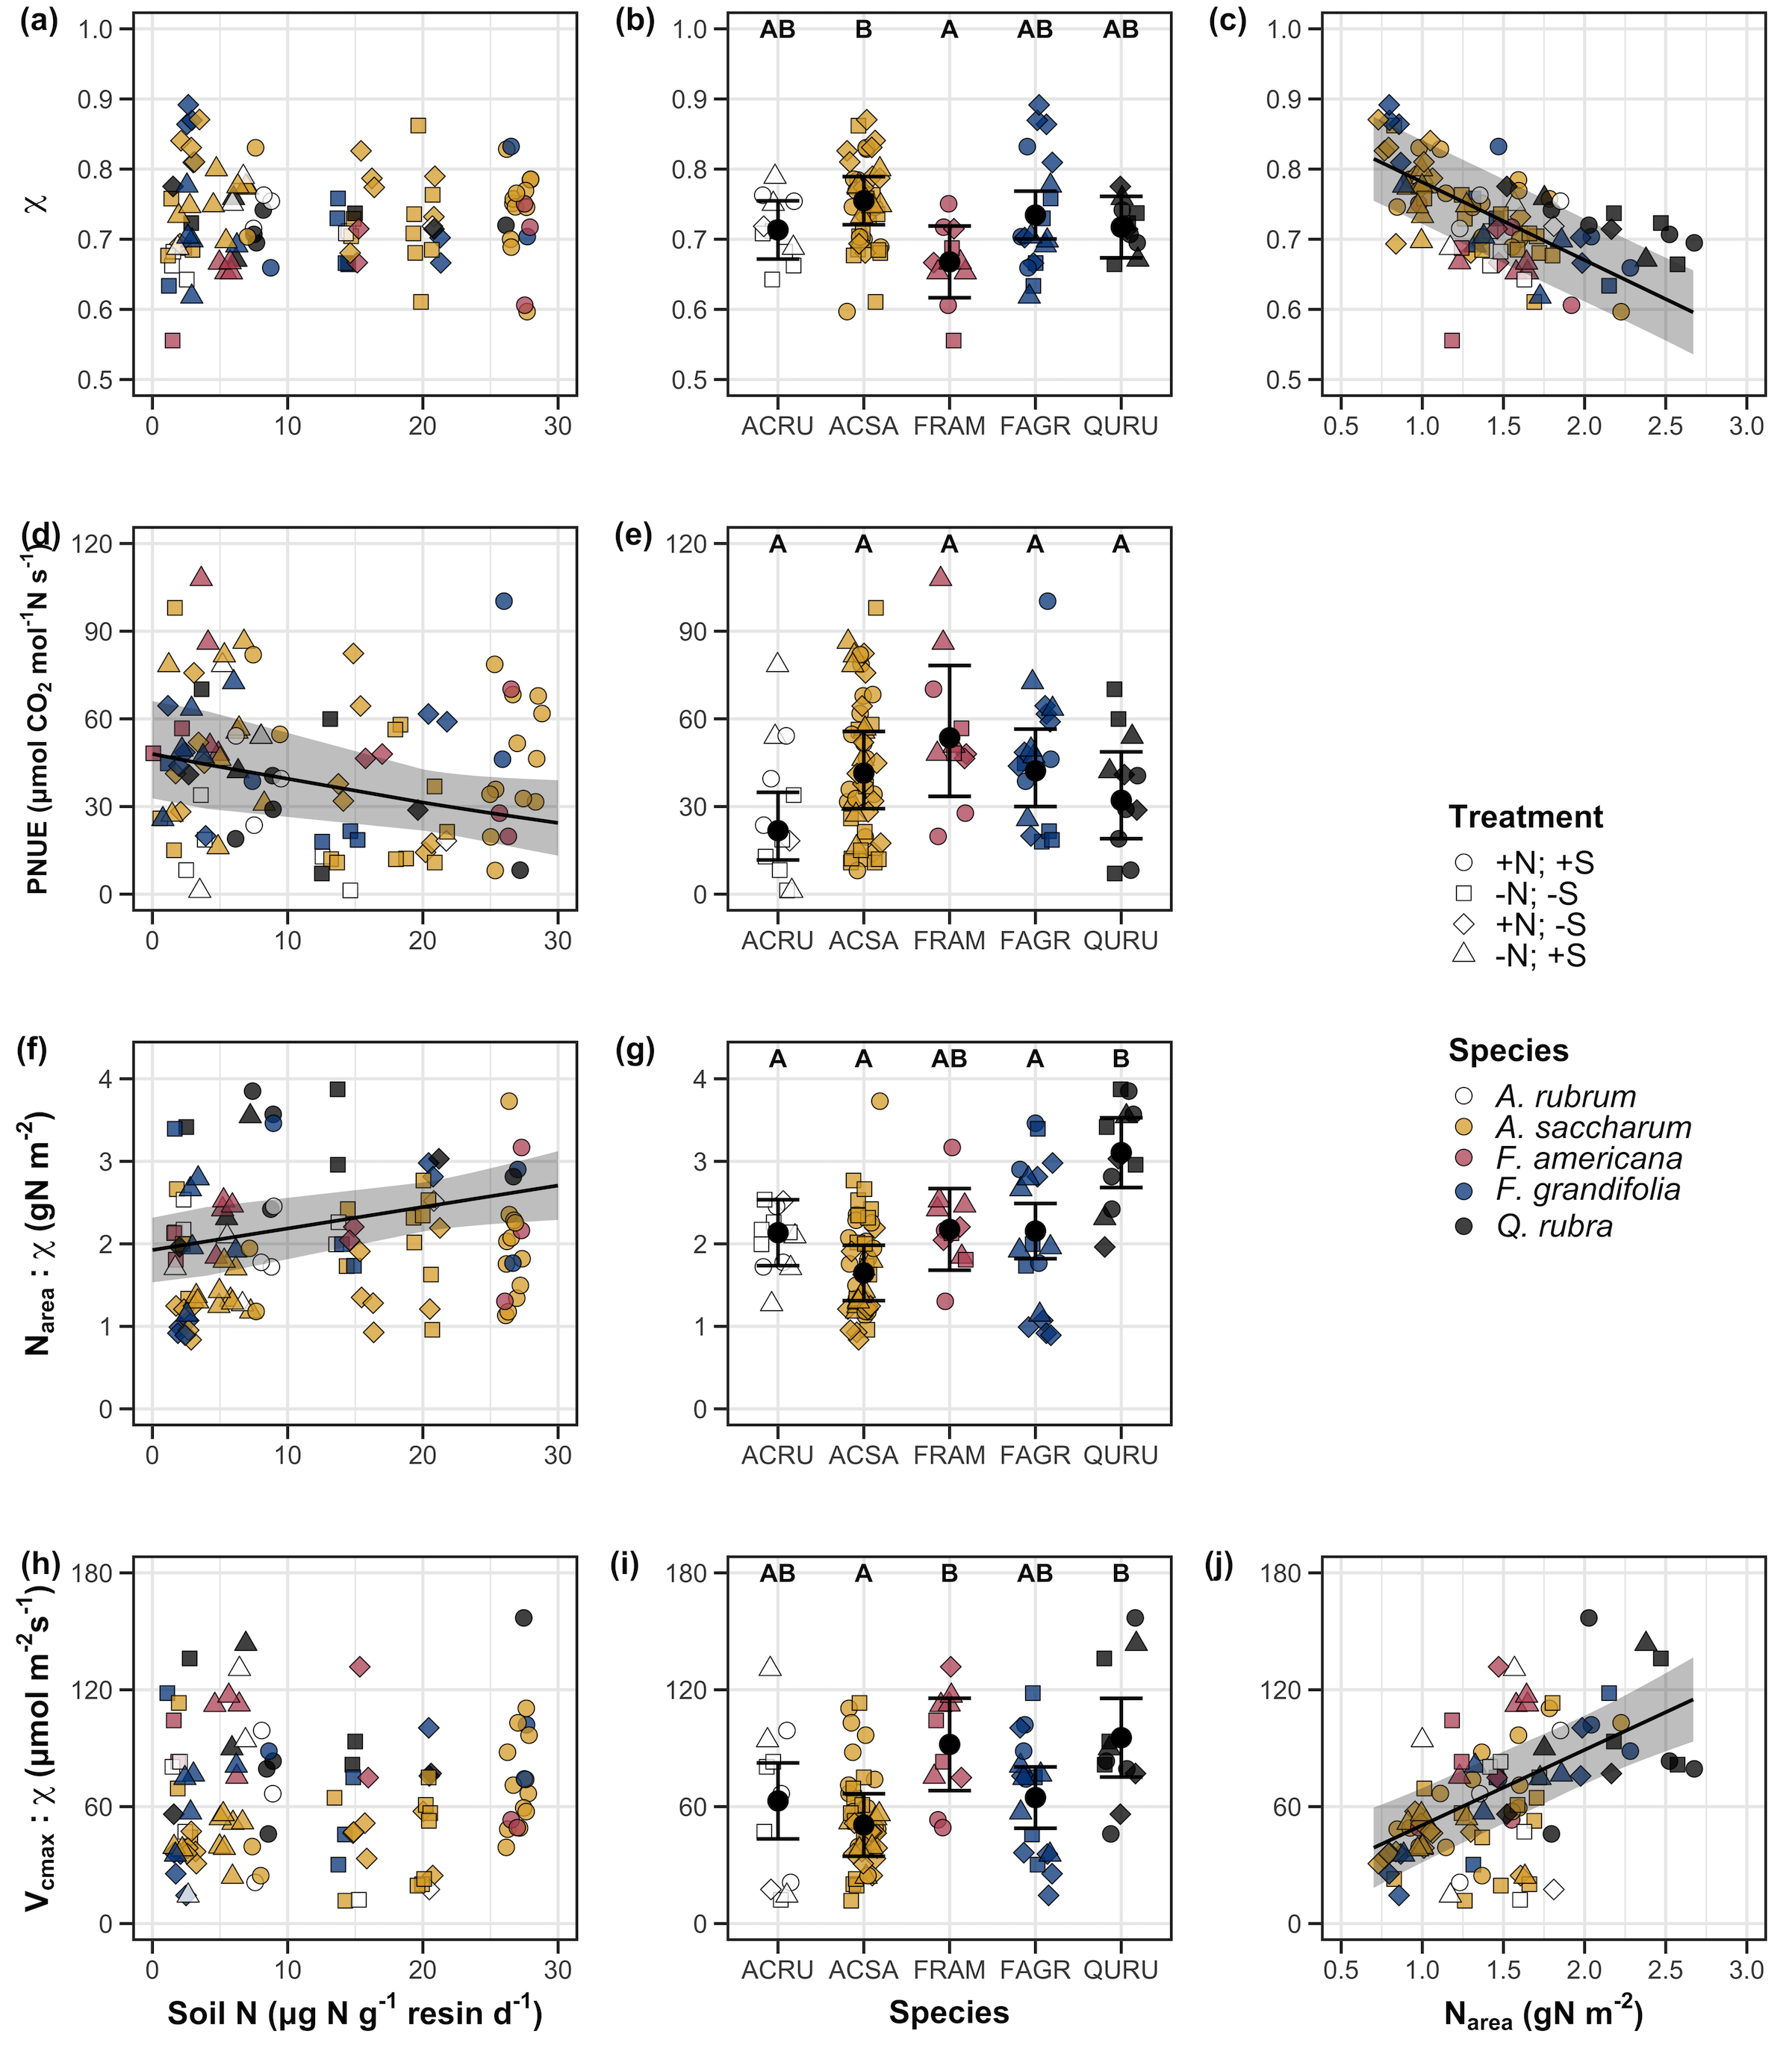
\includegraphics[width=\textwidth]{ch3_NxpH/figs/NxS_fig4_pnueiwue.png}
    \centering
    \caption[Effects of soil N availability, species, and leaf N content on tradeoffs between nitrogen and water use]{Effects of soil nitrogen availability and species on the proportion of leaf nitrogen content allocated to Rubisco (a-b), bioenergetics (c-d), photosynthesis (Rubisco + bioenergetics; e-f), and structure (g-h). Soil nitrogen availability is represented on the x-axis in the left column of panels and species are represented on the x-axis in the right column of panels. Species abbreviations and position along the x-axis in the middle column of panels, colored points, shapes, trendlines, error bars, and compact lettering are as explained in Figure \ref{fig:figure3.1}.}
    \label{fig:figure3.4}
\end{figure}
\clearpage

\section{Discussion}
\noindent Photosynthetic least-cost theory provides an explanation for understanding relationships between soil nutrient availability, leaf nutrient allocation, and photosynthetic capacity. The theory suggests that plants acclimate to a given environment by optimizing leaf photosynthesis rates at the lowest summed cost of using nutrients and water \shortcite{Prentice2014,Wang2017,Smith2019,Paillassa2020}. The theory predicts that an increase in soil nutrient availability should allow similar photosynthesis rates to be achieved with increased leaf nutrient content and photosynthetic capacity (i.e., $V_\mathrm{cmax25}$ and $J_\mathrm{max25}$) at lower leaf $C_\mathrm{i}$:$C_\mathrm{a}$ ($\chi$), resulting in an increase in water use efficiency, decrease in nutrient use efficiency, and increase in both leaf nutrient content and photosynthetic capacity per unit $\chi$. The theory predicts similar leaf responses to increasing soil pH under acidic conditions, presumably due to generally faster nutrient cycle dynamics and consequent reductions in the cost of acquiring nutrients relative to water with increasing soil pH \shortcite{Wang2017,Paillassa2020,Dong2020}.
    
Supporting the theory, increasing soil nitrogen availability was associated with increased leaf nitrogen content, a pattern that reduced photosynthetic nitrogen use efficiency and increased leaf nitrogen content per unit $\chi$. Increasing soil nitrogen coincided with slight, but non-significant decreases in $\chi$ and increases in $V_\mathrm{cmax25}$ and $J_\mathrm{max25}$ (\textit{p}<0.2, Table \ref{tab:table3.2}). The positive trend between soil nitrogen availability and photosynthetic capacity was supported by the concurrent strong increase in leaf nitrogen content with increasing soil nitrogen availability, which resulted in no change in the proportion of leaf nitrogen content allocated to photosynthesis across the soil nitrogen availability gradient. Additionally, leaf nitrogen content exhibited a strong negative correlation with $\chi$, indicative of strong nitrogen-water use tradeoffs at the leaf level. Responses tended to vary more due to soil nitrogen availability than soil pH. Overall, these findings are consistent with the nutrient-water use tradeoffs predicted from theory.

\subsection{\textit{Soil nitrogen availability modifies tradeoffs between nitrogen and water use}}
\noindent In support of expected least-cost outcomes and past environmental gradient studies \shortcite{Dong2017,Paillassa2020}, increasing soil nitrogen availability was associated with increased leaf nitrogen content. Soil nitrogen availability had smaller impacts on measures of net photosynthesis and $\chi$, which led to reductions in PNUE and increases in leaf nitrogen content per unit $\chi$, as expected from theory. Photosynthetic least-cost theory suggests that reductions in PNUE should be driven by an increase in the proportion of leaf nitrogen allocated to photosynthetic tissue, a pattern that should allow plants to achieve optimal photosynthetic rates with greater photosynthetic capacity to make better use of available light. Contrasting theory predictions, I found no effect of soil nitrogen availability on photosynthetic capacity. However, photosynthetic capacity did tend to increase with increasing soil nitrogen availability (\textit{p}<0.20; Table \ref{tab:table3.2}) resulting in no effect of soil nitrogen availability on the relative fraction of leaf nitrogen allocated to photosynthesis, Rubisco, or bioenergetics. These lines of evidence support the idea that trees use additional nitrogen to support increased leaf nitrogen allocation toward photosynthetic tissue and enhance photosynthetic capacity \shortcite{Wright2003}.

Soil nitrogen availability had a stronger effect on leaf nitrogen than photosynthetic capacity. This pattern suggests that additional plant nitrogen uptake due to increased soil nitrogen availability was also being used to support non-photosynthetic nitrogen pools, possibly to structural tissue or stress-induced amino acid and polyamine synthesis \shortcite{Minocha2000,Onoda2004,Bubier2011}. While I found no change in the proportion of leaf nitrogen allocated to leaf structural tissue, the overall stimulation in leaf nitrogen content with increasing soil nitrogen availability suggests an increase in the net amount of nitrogen invested in leaf structural tissue along the nitrogen availability gradient. Importantly, leaf nitrogen allocated to structure was calculated using an empirical relationship between $M_\mathrm{area}$ and the amount of leaf nitrogen allocated to cell walls \shortcite{Onoda2017}. As the generality of relationships between $M_\mathrm{area}$ and the amount of leaf nitrogen allocated to cell walls has been called into question \shortcite{Harrison2009}, future work should consider explicitly measuring nitrogen allocation to cell wall tissue and stress-induced amino acid synthesis to confirm these patterns.
    
In opposition to patterns expected from least-cost theory, increasing soil nitrogen availability had no apparent effect on $\chi$. Interestingly, despite the null effect of soil nitrogen availability on $\chi$, I observed a strong negative effect of increasing $N_\mathrm{area}$ on $\chi$, consistent with the nitrogen-water use tradeoffs expected from theory. The null response of $\chi$ to increasing soil nitrogen availability may have been due to a lack of water limitation in the system, given that the area received approximately 20\% more precipitation (1167 mm) during the 12-month period leading up to our measurement period than normally expected (972 mm). However, droughts can and do occur in temperate forests of the northeastern United States \shortcite{Sweet2017}, so the observed increase in leaf nitrogen content with increasing soil nitrogen availability could be a strategy that allows trees to hedge bets against drier than normal growing seasons \shortcite{Onoda2004,Onoda2017,Hallik2009}. As was suggested in \shortciteN{Paillassa2020}, and more recently by \shortciteN{Querejeta2022}, negative effects of soil nitrogen availability on $\chi$ may increase with increasing aridity. This strategy would be especially advantageous if it allows individuals growing in arid regions to maintain carbon assimilation rates with reduced water loss. Future work should attempt to quantify interactive roles of climate and soil nitrogen availability on nitrogen-water use tradeoffs, which could be done by leveraging coordinated and multifactor nutrient \shortcite{Borer2014} and water \shortcite{Knapp2017} manipulation experiments across broad climatic gradients.
    
\subsection{\textit{Soil pH did not modify tradeoffs between nitrogen and water usage}}
\noindent While the primary purpose of this study was to examine the role of soil nitrogen availability on nitrogen-water use tradeoffs, this experimental design manipulated both soil nitrogen and pH, providing an opportunity to isolate the roles of these variables. Previous correlational studies along environmental gradients have identified soil pH as a particularly important factor that can modify tradeoffs between nutrient and water use \shortcite{Smith2019,Paillassa2020,Westerband2023} and the proportion of leaf nitrogen allocated to photosynthesis \shortcite{Luo2021}. Such studies implied that these patterns may be driven by reductions in the cost of acquiring nutrients relative to water with increasing pH, which may be exacerbated in acidic soils.

Consistent with theory \shortcite{Wright2003,Prentice2014}, results indicate that increasing soil pH was negatively associated with PNUE. However, there was no effect of soil pH on leaf nitrogen content, $\chi$, or leaf nitrogen content per unit $\chi$, most likely because the experimental nitrogen additions increased soil nitrogen supply while both increasing (sodium nitrate) and decreasing (ammonium sulfate) soil pH. These results suggest that soil pH did not play a major role in modifying expected photosynthetic least-cost theory patterns, contrasting findings from \shortciteN{Paillassa2020} and other gradient studies that note positive effects of increasing soil pH on leaf nitrogen content, Rubisco carboxylation, and $\chi$ \shortcite{Viet2013,Cornwell2018,Luo2021}. Instead, null responses to soil pH show that leaf photosynthetic parameters depend more on soil nitrogen availability than pH per se, and that inferences from gradient studies might be confounding covariation between nitrogen availability and soil acidity.

\subsection{\textit{Species identity explains a large amount of variation in leaf and whole plant traits}}
\noindent Species generally explained a larger amount of variation in measured leaf traits than soil nitrogen availability or soil pH. Interspecies variation is an important factor to consider when deducing mechanisms that drive photosynthetic least-cost theory, particularly for species that form distinct mycorrhizal associations or have different photosynthetic pathways, growth forms, or leaf habit \shortcite{Espelta2005,Adams2016,BialicMurphy2021,Scott2022}. The need to consider species may also be important when comparing nutrient-water use tradeoffs in early and late successional species, or in species with different resource economic strategies \shortcite{Abrams1995,Ellsworth1996,Wright2004,Reich2014,Onoda2017,Ziegler2020}.
    
A strength of the study design and sampling effort is that it controls for many species differences that should modify nitrogen-water use tradeoffs expected from theory. All tree species measured in this study shared the leaf habit of deciduous broadleaves, were growing in forests of similar successional stage, but differed in mycorrhizal association and consequent resource economic strategies. As stands tended to be dominated by trees that associate with arbuscular mycorrhizae (\textit{Fraxinus} and both \textit{Acer} species made up roughly 70\% of total aboveground biomass across stands), ecosystem biogeochemical cycle dynamics may be more closely aligned to the inorganic nutrient economy proposed in \shortciteN{Phillips2013}, which may promote stronger nitrogen-water use tradeoffs in tree species that associate with arbuscular mycorrhizae. This result was not observed here, as photosynthetic properties varied as much within as across the two mycorrhizal associations represented. Given the high variability in measured photosynthetic traits within and across species, effects of mycorrhizal association likely require more intensive sampling efforts to detect than were possible here.
    
\subsection{\textit{Implications for photosynthetic least-cost theory model development}}
\noindent In the field, soil nutrient availability is heterogeneous across time and space (Table \ref{tab:table.b4}). Unaccounted within-plot heterogeneity may have contributed to the low amount of variation explained by soil nitrogen availability in statistical models, as resin bags are a coarse surrogate for soil nitrogen availability. Despite this, I still observed evidence for nutrient-water use tradeoffs, suggesting that observed responses reported here may be an underestimate toward the net effect of soil nitrogen availability on these tradeoffs. While I urge caution in the interpretation of these results, they do provide a promising baseline for future studies investigating patterns expected from photosynthetic least-cost theory at finer spatiotemporal resolutions.
    
The general stronger relationship between leaf nitrogen content and photosynthetic parameters versus between leaf nitrogen content and soil nitrogen availability suggests that leaf nitrogen content is more directly tied to photosynthesis than soil nitrogen availability. While this could be due to the high spatiotemporal heterogeneity of soil nitrogen availability, principles from photosynthetic least-cost theory suggest that leaf nitrogen content is the downstream product of leaf nutrient demand to build and maintain photosynthetic machinery, which is set by aboveground environmental conditions such as light availability, CO$_2$, temperature, or vapor pressure deficit \shortcite{Smith2019,Paillassa2020,Peng2021,Westerband2023}. The stronger relationship between leaf nitrogen and photosynthetic parameters, paired with the strong negative relationship between leaf nitrogen and $\chi$, could indicate a relatively stronger effect of climate on leaf nitrogen-photosynthesis relationships than soil resource availability. However, the short distance between plots and across sites limited my ability to test this mechanism.
    
Variation in soil pH affected least cost responses less than variations in soil nitrogen availability, in part because experimental treatments directly increased soil nitrogen and affected soil pH in opposite directions. While soil pH has been shown to drive nitrogen-water tradeoffs in global gradient analyses \shortcite{Viet2013,Paillassa2020}, these responses may be due to covariations between soil pH and nutrient cycling rather than a role of pH per se. The direct manipulations of soil pH and soil nitrogen availability in this study partly disentangle these factors and show that variation in nitrogen availability matters more for least-cost tradeoffs than pH alone.

\subsection{\textit{Conclusions}}
\noindent Increasing soil nitrogen availability generally increased leaf nitrogen content (both area- and mass-based), but did not significantly influence $\chi$. This shift in leaf nitrogen led to a reduction in PNUE, and an increase in leaf nitrogen per unit $\chi$ with increasing soil nitrogen availability. Despite null effects of soil nitrogen availability on $\chi$, I observed a strong negative relationship between leaf nitrogen content and $\chi$. These results provide empirical support for the nutrient-water use tradeoffs expected from photosynthetic least-cost theory in response to increasing soil nutrient availability, but suggest that all tenets of the theory may not hold in every environment. These results experimentally test previous work suggesting that leaf nitrogen-water economies vary across gradients of soil nutrient availability and pH, and show that variations in nutrient availability matter more for determining variation in leaf photosynthetic traits than soil pH.
